\documentclass{article}
\usepackage[utf8]{inputenc}

\title{DotA 2}
\author{David 'DaveTheMicrowave' Enderlin}
\date{\today}

\usepackage{natbib}
\usepackage{graphicx}
\usepackage{hyperref}

\begin{document}
	
	\makeatletter
	\begin{titlepage}
		\centering
		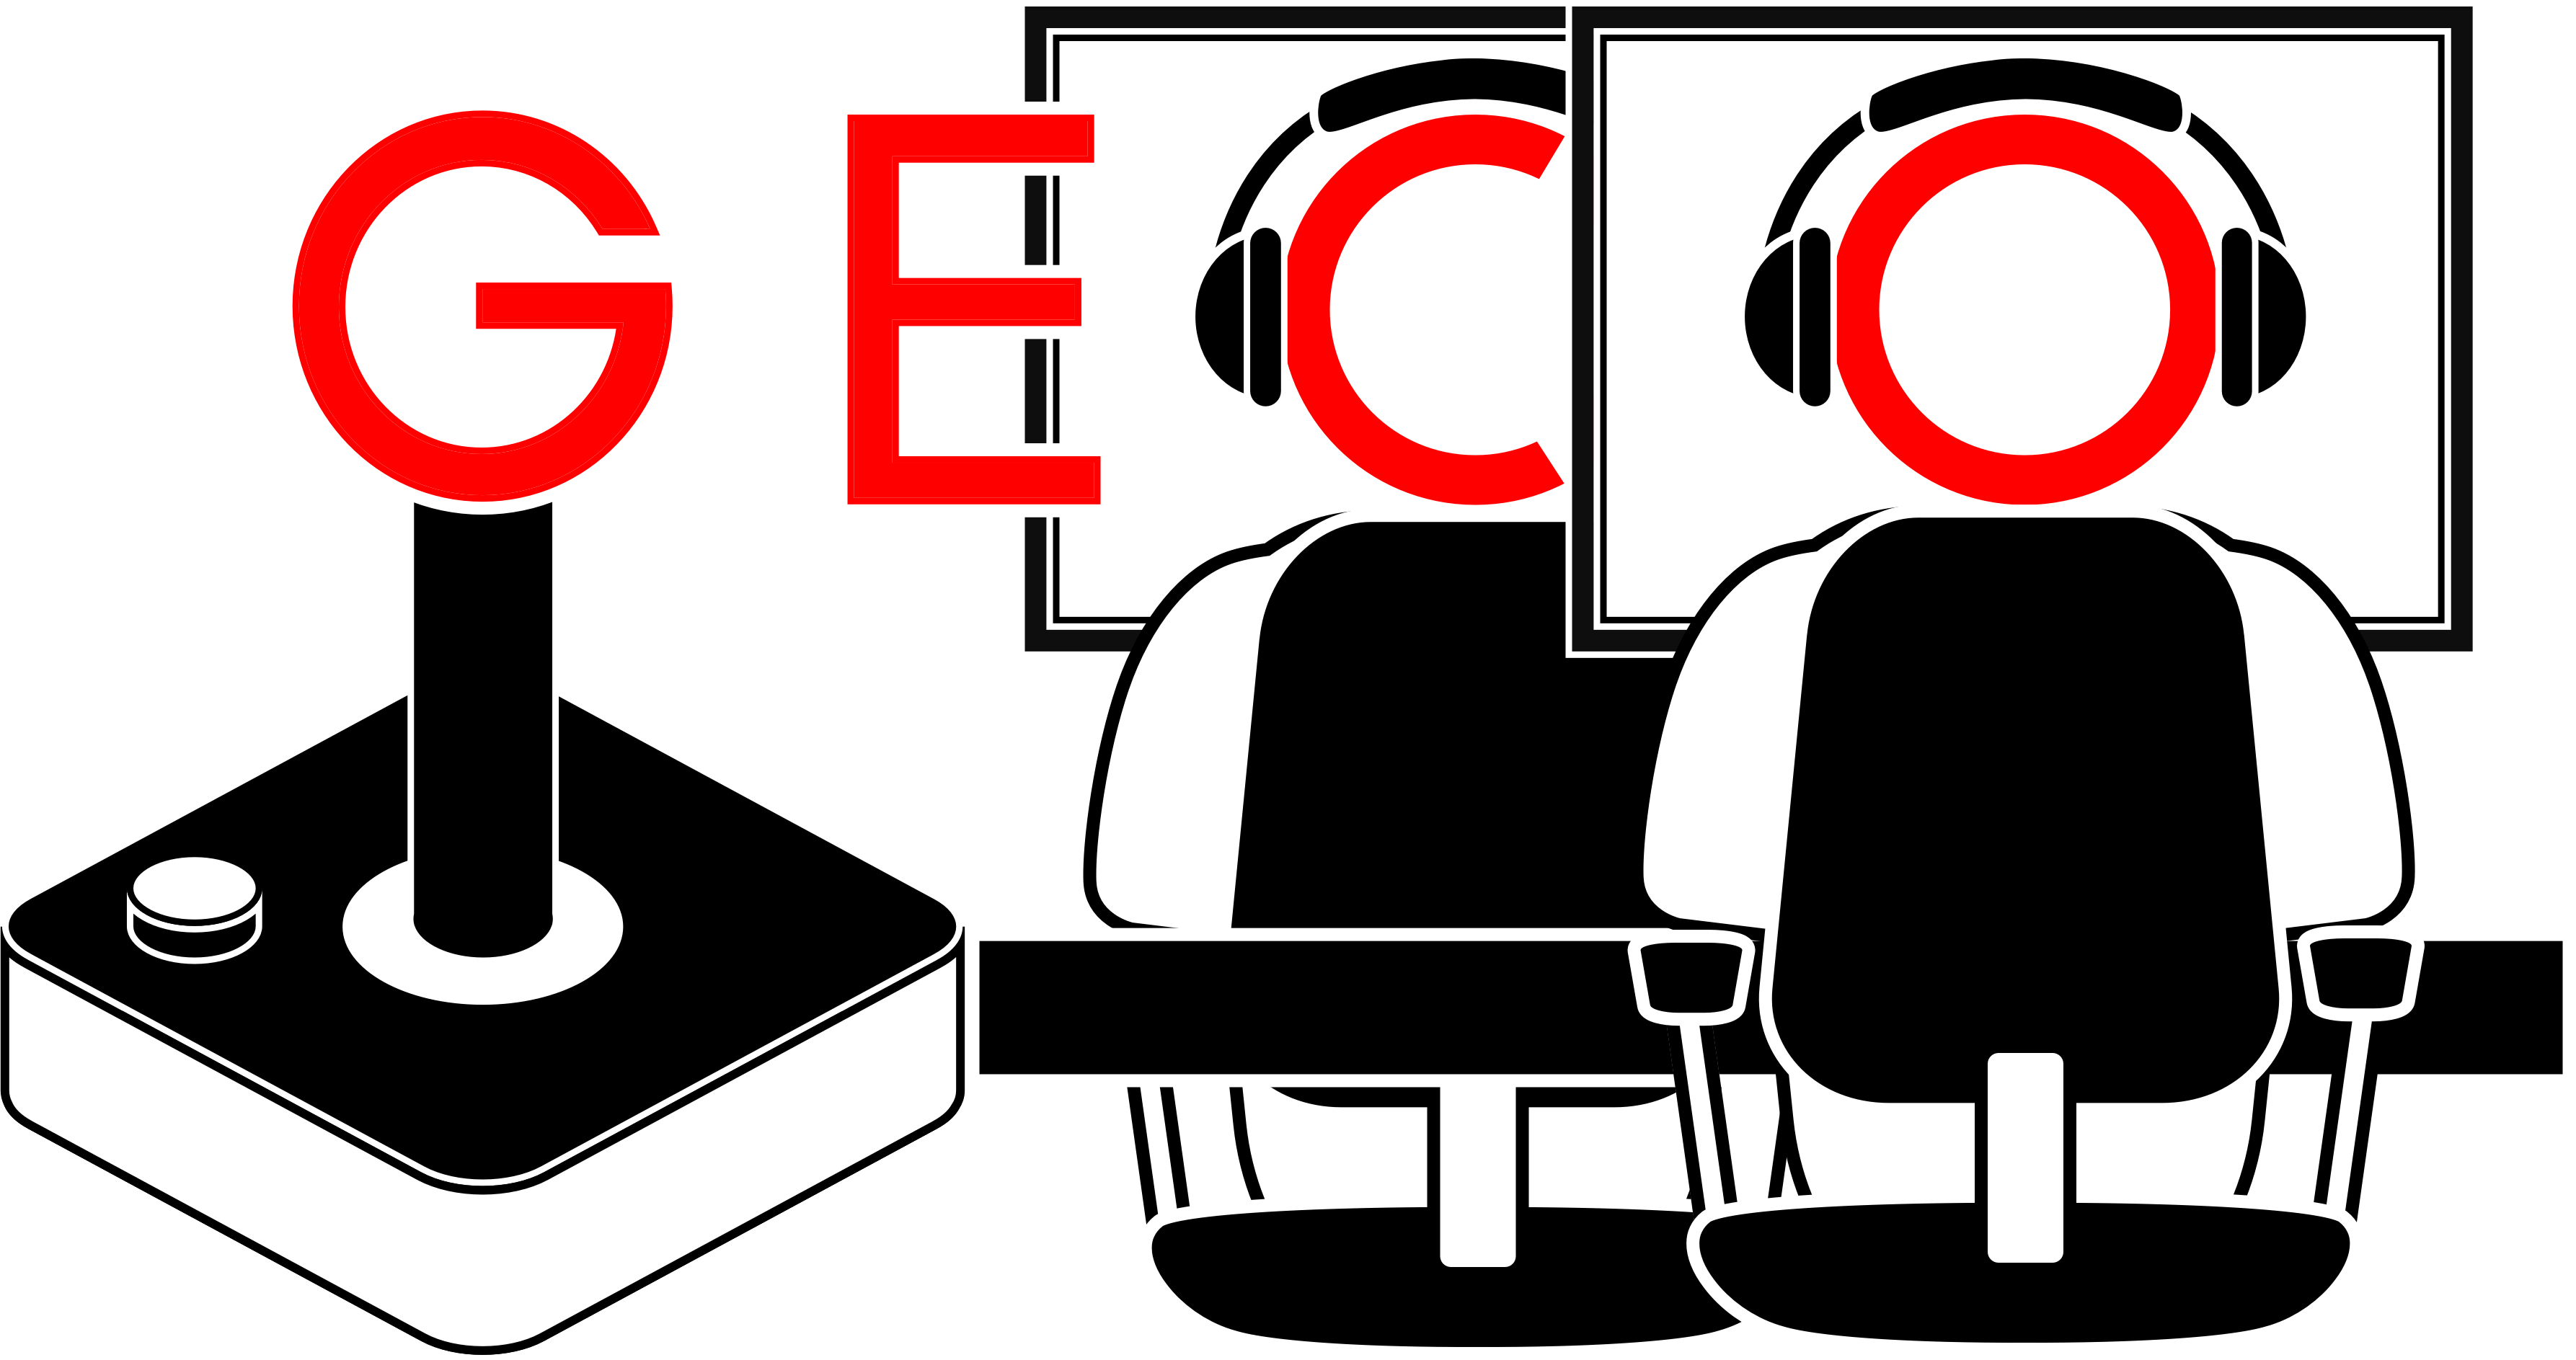
\includegraphics[scale=0.075]{GECo.png}\\
		\LARGE \@title\\ Tournament Rules\\ \normalsize by \@author\\ \@date
	\end{titlepage}
	\makeatother
	
	\clearpage
	
	\tableofcontents
	\clearpage
	
	\section{General Tournament Rules}
	Read the general tournament rules of the current event.\\
	All the general rules apply to this tournament.
	
	\section{Match format}
	The tournament uses the default competitive rule set of DotA 2, which means that the gamemode which is going to be played will be Captains Mode with all heroes which are allowed at the time of the tournament in Captains Mode.
	
	\section{Dota Plus}
	The plus assistant is \textbf{not allowed during the match} since it could give an advantage over people without it. It is however \textbf{allowed in the pick-phase} since it's not possible to disable the assistant in the pick-phase. If someone of your team uses the plus assistant \textbf{during} the match, your team will be disqualified for that match. Before each match, make sure that you \textbf{don't select} the plus assistant as hero guide and disable the option \textit{"Use Plus Assistant rather than the default guides"} in the advanced options.
	
	\section{Matches}
	\subsection{Side}
	If both teams don't agree on which sides they play, they will decide it at random for example by flipping a coin. 
	
	\subsection{Server}
	The lobbies for the games will be created by one of the teams. The exact settings for the lobbies will be provided at the LAN Party but they will be close to the default competitive settings. 
	
	\subsection{Pause}
	Pausing is allowed if there are any technical problems and if it's not during a teamfight. After pausing, you immediately have to state the reason for your pause in all chat. Pausing for tactical reasons or during a teamfight is not allowed and could disqualify your team for the current match. If you think a pause was not justified, please contact an admin.
\end{document}
